\begin{figure}[h!]
	\centering
	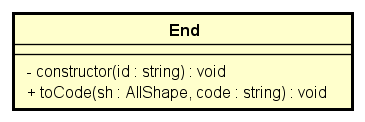
\includegraphics[scale=0.8]{res/sections/SpecificaFrontEnd/Services/Disegnetti/end.png}
	\caption{Diagramma della classe End}
\end{figure}

\begin{itemize}
	\item \textbf{Descrizione:}\\
	
	\item \textbf{Utilizzo:}\\
	
	\item \textbf{Metodi:}
		\begin{itemize}
			\item \emph{-constructor(id : string)}\\
    		\\
    		\textbf{Parametri:}
    		\begin{itemize}
    			\item \emph{id : string}\\
    			
    		\end{itemize}
			\item \emph{+getType())}\\
    		
			\item \emph{+toCode(sh: AllShape, code: string)}\\
    		\\
    		\textbf{Parametri:}
    		\begin{itemize}
    			\item \emph{sh: AllShape}\\
    			
    			\item \emph{code: string}\\
    			
    		\end{itemize}
    	\end{itemize}
\end{itemize}